%% LyX 2.0.5.1 created this file.  For more info, see http://www.lyx.org/.
%% Do not edit unless you really know what you are doing.
%\documentclass[12pt,english]{report}
%\usepackage{mathptmx}
%\renewcommand{\familydefault}{\rmdefault}
%\usepackage[T1]{fontenc}
%\usepackage[latin9]{inputenc}
%\usepackage[a4paper]{geometry}
%\setcounter{secnumdepth}{2} % Changed from 3 to 2. 0-chapter 1-section 2-subsection 
%\setcounter{tocdepth}{2} % Changed from 3 to 2. 0-chapter 1-section 2-subsection 
%\setlength{\parskip}{\medskipamount}
%\setlength{\parindent}{0pt}
%\usepackage{verbatim}
%\usepackage{pdfpages}
%\usepackage{graphicx}
%\usepackage{subfig} %% This package has to be here
%\usepackage{setspace}
%\usepackage{arabtex}
%\usepackage[numbers]{natbib}
%\usepackage{nomencl}
%\usepackage{amsthm}
%\usepackage{amsmath}
%\usepackage{amsfonts}
%\usepackage{paralist}
%\usepackage{etoolbox}
%\newtoggle{edit-mode}
%\toggletrue{edit-mode}  
%%%\toggletrue{edit-mode}
%\iftoggle{edit-mode}{
%\geometry{verbose,tmargin=2cm,bmargin=2cm,lmargin=2cm,rmargin=6cm,headheight=1cm,headsep=1cm,footskip=1cm, marginparwidth=5cm}
%}{
%\geometry{verbose,tmargin=2cm,bmargin=2cm,lmargin=2cm,rmargin=2cm,headheight=1cm,headsep=1cm,footskip=1cm}
%}
%
%
%\begin{document}

%%%%%%%%%%% nomenclature %%%%%%%%%%
\nomenclature{HWR}{Handwriting Recognition}
\nomenclature{OCR}{Optical Character Recognition}
\nomenclature{WP}{Word Part}
\nomenclature{ANN}{Artificial Neural Network}
\nomenclature{SVM}{Support Vector Machine}
\nomenclature{$k$-NN}{$k$ Nearest Neighbours}
\nomenclature{SP}{Segmentation Point}
\nomenclature{POI}{Point Of Interest} 
%%%%%%%%%%%%%%%%%%%%%%%%%%%%%%%%%%%%

\chapter{Introduction}

\section{Background and Previous Work}

\subsection{Handwriting Recognition}
\iftoggle{edit-mode}{\hspace{0pt}\marginpar{HWR Motivation 1 - handwriting importance and survival}}{}
Writing has made much of the culture and civilization possible.
It was developed as a mean to expand human memory and to facilitate communication. 
Converting handwritten script into its digital analogous is highly motivated by the ease and convenience of the digital representation.
Not only this is useful for making digital copies of handwritten documents, but also in many automated processing tasks such as searching, indexing, automatic mail sorting, editing, sharing, and more \cite{noaparast2009persian,connell2000online}. 

\iftoggle{edit-mode}{\hspace{0pt}\marginpar{HWR as OCR}}{} 
\emph{Handwriting recognition} (HWR) was defined by Plamondon and Srihari \cite{plamondon2000online} as "the task of transforming a language represented in its spatial form of graphical marks into its symbolic representation".
In contrast to HWR, \emph{Optical character recognition} (OCR) targets recognising typewritten text.
OCR and HWR are important areas in the pattern recognition field. 
Both areas have been steadily evolving during their history and have always been a favourite testing ground for new ideas in pattern recognition, giving rise to an exciting set of research topics and producing many powerful practical applications.
However, since many experiments of new ideas in pattern recognition were conducted on isolated characters, the results are not always immediately reflected in HWR applications \cite{burrow2004arabic}.
Although considered a well developed technological field, HWR remains an areas of active scientific research and creative engineering \cite{borovikov2004survey}.
Besides recognition, handwriting is associated with other types of analysis, such as signature verification, writer identification, etc.

\iftoggle{edit-mode}{\hspace{0pt}\marginpar{Levels of difficulties in HWR}}{}
There are different types of problems with varying complexity within the HWR field.
In one extreme there is the case of isolated characters written inside graphical boxes in which the segmentation problem is already solved. The opposite extreme is the case of cursive unrestricted handwriting in which words or portions of a word are written with a single stroke using ligatures that connect adjacent letters. 
HWR systems have a strong history in making use of this graduation in difficulty \cite{bahlmann2005advanced}. 

\iftoggle{edit-mode}{\hspace{0pt}\marginpar{Arabic HWR challenge}}{}
A script is a set of icons that have certain basic shapes. 
These are known as characters or letters.
Each script has its own rules regarding how letters are combined to form shapes that represent higher level linguistic units \cite{plamondon2000online}.
Unlike the Latin script, in which non-cursive handwriting is possible and common, Arabic is cursively written in both handwritten and printed text.
Its unconstrained nature, which produces a huge variety in the handwriting of different people, makes the recognition of Arabic script extremely difficult.
Figure \ref{fig:ha_different} shows several handwritten samples the letter \RL{.h} /.h/, in its isolated form, written by several writers.

Text segmentation, that is, the process of dividing a cursive writing into sub-units (typically characters) turns out to be a challenging task.

\begin{figure}
\centering
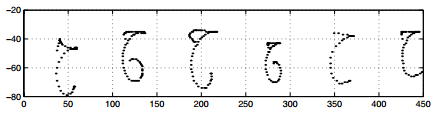
\includegraphics{./figures/ha_different}       
\caption{Different writing styles of the isolated form of the letter \RL{.h} /.h/.}
\label{fig:ha_different}
\end{figure}


%%%%%%%%%%%%%%%%%%%%%%%%%%%%%%%%%%%%%%%%%%%%%%
\subsection{Off-line versus On-line Handwriting Recognition}

\iftoggle{edit-mode}{\hspace{0pt}\marginpar{Introduction}}{}
The field of HWR can be classified in several ways, however, the most common categorization is the one that distinguishes between \emph{off-line} (also called static) and \emph{on-line} (also called dynamic).
Off-line HWR focuses on documents that have been written on paper at some previous point of time. 
A digital image of the document, represented as a raw 2-dimensional pixel data, is fed to the computer and the system attempts to convert the spatial representation of the letters into digital symbols \cite{al2011online}. 
In contrast, on-line HWR is performed on a digital representation of the text written on a special digitizer, tablet or smart-phone device, where sensors pick up the pen-tip movements and the two-dimensional coordinates of successive points of the writing as a function of time are stored. 

\begin{figure}
	\centering
        \subfloat[]{
            \label{fig:offline}
            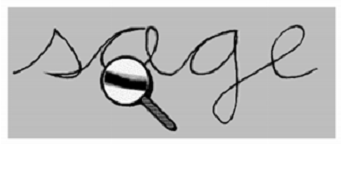
\includegraphics[width=0.5\textwidth]{./figures/offline}
        }
        \subfloat[]{
           \label{fig:online}
           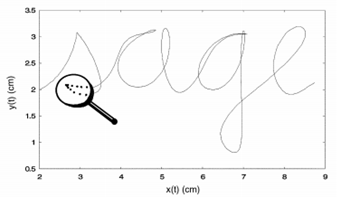
\includegraphics[width=0.5\textwidth]{./figures/online}
        }        
    \caption{An on-line vs. an off-line representation of a word \cite{plamondon2000online}.}
   \label{fig:offline_vs_online}
\end{figure}

\iftoggle{edit-mode}{\hspace{0pt}\marginpar{Similarities and advantages of on-line and off-line}}{}
Off-line HWR techniques can be applied to on-line data by constructing a static image of the on-line script. 
However, it has been shown that the information of the pen dynamics, such as the strokes breaking (i.e., "pen-down" and "pen-up" events) and the order of writing, can be used to obtain a better recognition accuracies than the static data alone. 
In the other direction, the success of on-line systems makes it attractive to consider developing off-line systems that first estimate the trajectory of the writing from the off-line data and then use on-line HWR techniques. 
Nevertheless, reconstructing the temporal data is problematic, and thus, has led to few such systems so far \cite{plamondon2000online}.

\iftoggle{edit-mode}{\hspace{0pt}\marginpar{off-line objectives}}{}
In general, off-line HWR systems are less accurate than on-line systems, but, they are now good enough that they have a significant economic impact on specialized domains such as interpreting handwritten postal addresses on envelopes and reading courtesy amounts on bank checks \cite{melin2007analysis}.

\iftoggle{edit-mode}{\hspace{0pt}\marginpar{A general flow for HWR}}{}
Despite the large variation among the different methods for HWR, there are several fundamental stages that are common between most of the systems.
The data acquisition step is the first stage in HWR. 
In the on-line case, the stylus motion is usually sampled at equal time intervals.
The samples go through a preprocessing stage that includes filtering, re-sampling, and normalization. 
Additional preprocessing may include slant and slope corrections. 
Then, depending on the nature of the system, the script may undergo segmentation into basic units that could be words, parts of words, single characters or graphemes.
Typically, a feature extraction technique is then applied to extract significant and distinguishing attributes of the input data.
Finally, using a classification algorithm the basic units are labelled. 
In many implementations, a post-processing stage is applied in which the language model is used to search for the most likely string in the lexicon.

\iftoggle{edit-mode}{\hspace{0pt}\marginpar{off-line HWR additional steps}}{}
Approaches for on-line and off-line handwriting recognition, while having much in common, are different, due to the disparity in the input data representation. 
Their different nature imposes different challenges and thus variable levels of efforts are required to be spent on the various stages.
The off-line HWR systems usually consist of additional steps of layout analysis and text lines extraction, which are activated at the beginning of the preprocessing stage. 
Each text line is then divided into words or parts of words. 
The segmentation, in such system, is made into images that contain basic units. 
The whole process is straightforward for well printed or well written documents; however, in the case of historical or badly printed document much effort is invested in a preprocessing stage that include smoothing, writing flow reconstruction, purification, and more \cite{saba2010survey}. 

\iftoggle{edit-mode}{\hspace{0pt}\marginpar{Literature}}{}
The research on on-line handwriting recognition started in the 1960's and has been receiving a great interest from the 1980's \cite{tagougui2013online}.
One of the earliest studies on on-line Arabic script recognition was carried out by El-Wakil and Shoukry in 1989 \cite{el1989line}.

%%%%%%%%%%%%%%%%%%%%%%%%%%%%%%%%%%%%%%%%%%%%%%

\subsection{Holistic versus the Analytic Approaches}

\iftoggle{edit-mode}{\hspace{0pt}\marginpar{Importance of the dictionary size}}{}
The vocabulary from which the word samples are taken, has a major impact on how difficult the HWR task is.
Closed-vocabulary HWR systems are capable of recognizing words from a predetermined limited size dictionary which usually called a lexicon.
There are no well-established criteria for the categorization of lexicon size. 
However, a lexicon that contains tens of words is considered a small lexicon and a lexicon t hat contains tend of thousands of words is considered a very large lexicon.
Open-vocabulary systems refer to such that recognize any word without the constraint of being in a dictionary.
The lexicon is a key-point post-processing stage in many systems, because the linguistic knowledge helps to filter out many possible options that are not included in the lexicon, and consequently raises the recognition rate.
The adhesion to a limited dictionary, may also limit the computational complexity. 
Although most research efforts have been devoted to closed vocabulary systems, open vocabulary systems have also been proposed.
Yet, their accuracy is still far below those relying on a small vocabulary \cite{koerich2003large, shu1996line}.

\iftoggle{edit-mode}{\hspace{0pt}\marginpar{problems imposed by the open vocabulary}}{}
While there exists a wide variety of approaches to cursive script recognition, research in this field has established two main approaches, one is the analytic approach \cite{abdulla2008off, sari2002off, dinges2011offine, elanwar2012unconstrained}, and the other is the holistic approach \cite{biadsy2011segmentation}. 


The analytic approach involves segmentation of the input curve into basic units and the classification of each individual unit.
The advantage of this approach is that it requires to maintain only a small set of trained models - one for each letter shape - to handle large vocabulary. 
However, the absence of consistent baselines, large variations in writing styles, and seamless connection between letters (connection is done with almost no ligatures) makes segmentation into individual letters very challenging \cite{saabni2009hierarchical}.

\iftoggle{edit-mode}{\hspace{0pt}\marginpar{The holistic approach}}{}
The holistic approach considers the global properties of the written text and recognizes the input word shape as a whole, avoiding errors in the segmentation process. 
The limitation of this approach is that the classifier needs to be trained over all words in the dictionary and to maintain and train models for each word.
Employing the holistic approach may be possible for a small vocabulary of words, however, this is not feasible for large vocabularies (20,000 words or more).

A survey done in \cite{al2011online} on Arabic HWR found that the analytic approach, in general, achieve higher recognition rates than the holistic systems, in cases where words are written in cursive manner, such in the Arabic script. 

%%%%%%%%%%%%%%%%%%%%%%%%%%%%%%%%%%%%%%%%%%%%%%%%%%%%%%%

\subsection{The Arabic Language}

\iftoggle{edit-mode}{\hspace{0pt}\marginpar{The Arabic spread}}{}
The Arabic script is a descendant of its Aramaic ancestor. 
The earliest known document written using the Arabic script dates from 512 AD.
Arabic is spoken, as their first language, by nearly 350 million people around the world, and written by more than 100 million people, in over 20 different countries \cite{zeki2011segmentation}.
It is one of the five most common languages in the world and one of the six official languages of the united nations since 1974 \cite{burrow2004arabic}. 
Although Arabic is used mainly in the Arab countries, which consists of about 5.5\% of the world population, almost all Muslims, around 25\% of the world population can read Arabic script as it is the language of the Holy Qur'an \cite{zeki2011segmentation}.

\iftoggle{edit-mode}{\hspace{0pt}\marginpar{The Arabic Alphabet usage in other languages}}{}
The use of the Arabic language extended in the $7^{th}$ and $8^{th}$ centuries from India to the Atlantic ocean due to the Islamic conquests \cite{saabni2009efficient}. 
Consequently, more than twenty different languages adopted the Arabic alphabet with some changes. 
Examples are Farsi, Urdu, Malay, Housa and Ottoman Turkish.
Nevertheless, some of those languages has later adopted the Latin characters, but in general, people can still read the Arabic script \cite{zeki2011segmentation}.

\iftoggle{edit-mode}{\hspace{0pt}\marginpar{Literary vs. daily language}}{}
Although spoken Arabic is different from country to country, written Arabic is a standard system used all over the Arab world.
The literary language is called \emph{modern standard Arabic} or \emph{literary Arabic}.
It is the only official form of Arabic used in most written documents as well as in formal spoken occasions, such as lectures and news broadcasts. 

\iftoggle{edit-mode}{\hspace{0pt}\marginpar{The growing interest in the Arabic HWR}}{}
Arabic HWR research came to the attention of researchers very recently compared to Latin and Chinese.
The first work on Arabic character recognition is by Nazif \cite{nazif1975system} published in 1975, while the earlier research efforts in Latin may be traced back to the middle of the 1940s.
However, considerable increase in the number of research papers related to Arabic character recognition is evident in recent years.
The challenging nature of the Arabic HWR has attracted the attention of researchers from industry and academic circles \cite{al2010development, zeki2011segmentation}.
A recent survey done by Tagougui et al. \cite{tagougui2013online} reviews the status of research in the on-line Arabic HWR field. 

\subsubsection{Characteristic of the Arabic Writing System}
\label{subsubsec:arabic_writing_characteristic}

\iftoggle{edit-mode}{\hspace{0pt}\marginpar{Basic properties}}{}
The Arabic script consists of 28 basic letters.
It is written from right to left in a semi-cursive manner in both printed and handwritten forms.
Most letters are written in four different letter shapes depending on their position in the word, e.g., the letter \RL{`} /ain/ appears as \RL{`}  in its isolated form, \RL{`-} in its initial form, \RL{-`-} in its medial form and \RL{-`} in it final form. 
Among the basic letters, six are dis-connective - \RL{A} /a/, \RL{d} /d/, \RL{_d} /th/, \RL{r} /r/  \RL{z} /z/ and \RL{w} /w/. 
Dis-connective letters do not connect to the following letter and have only two shapes, isolated and final. 
The presence of these letters interrupts the graphic continuity of a word. 
The graphically connected parts of the word are called \emph{word parts} (WPs) \cite{biadsy2011segmentation}. 

\iftoggle{edit-mode}{\hspace{0pt}\marginpar{Delayed strokes}}{}
Dots and strokes used in the Arabic script are called \emph{delayed strokes} or \emph{additional strokes} and are usually drawn last when scribing a WP or a word. 
There are mainly two types of delayed strokes, \emph{i'jam} (\RL{A`jAm}) and \emph{harakat} (\RL{.hrkAt}). 

\iftoggle{edit-mode}{\hspace{0pt}\marginpar{I'jam}}{}
The i'jam are the pointing diacritics added to the main body of the letter, called \emph{rasm} (\RL{rsm}), and their role is to distinguish between various constants, such as the medial form letters \RL{-b-} /b/, \RL{-t-} /t/, \RL{-_t-} /s/, \RL{-n-} /n/, \RL{-y-} /y/.
Typically, i'jam are not considered diacritics but part of the letter and consists of one or more dots and lines added above, under or inside the letter.
Eliminating, adding or moving a i'jam produces a completely different letter and as a result a completely different word, thus, they are not omitted in the written documents.
In addition to the frequently used dots, the \RL{'} (hamza) is another type of i'jam that distinguish between the letters \RL{k} /k/ and \RL{l} /l/ in their isolated and final forms.

\iftoggle{edit-mode}{\hspace{0pt}\marginpar{Harakat}}{}
The harakat are small markings added above or below the letters, are used to specify the exact pronunciation of the word.
These diacritics are used in the holy book Qur'an and are frequently used in teaching material and poetry but are seldom used in day-to-day communication and handwriting neither are much in use in the scientific and business communication.

The old Arabic was written without dots or diacritics. 
These additional strokes were added around the 7th century, to prevent the Qur'an from being misread by Muslims \cite{burrow2004arabic}.
An example of a fully vocalised Arabic from the Qur'an (Al-Fatiha 1:1):
\begin{center}
\fullvocalize
\transtrue
\begin{RLtext}
bismi al-ll_ahi al-rra.hm_ani al-rra.hImi
\end{RLtext}
In the name of All'ah, the most gracious, the most merciful.
\end{center}

\iftoggle{edit-mode}{\hspace{0pt}\marginpar{additional stroke}}{}  
In our work we recognize and classify the main body of the letter and ignore the additional stroke entirely (both i'jam and harakat). 
As a result, the number of different letters drops from $28$ to $18$.
It is important to note that taking the delayed strokes into consideration may be exploited to boost the classification rate.
See Table \ref{table:same_body_letters} for identical rasm Arabic letters.

\iftoggle{edit-mode}{\hspace{0pt}\marginpar{WP count}}{}    
Saabni and El-sana \cite{saabni2009efficient} have explored a large collection of Arabic texts and extracted $300,000$ different word combinations of $82,000$ different WPs.
Ignoring the delayed strokes, the number of different WP had reduced to $40,000$.

\iftoggle{edit-mode}{\hspace{0pt}\marginpar{Challenges of the Arabic language}}{}  
There are several complexities that arise when attempting to recognize Arabic Script.
First, while the main body of most Arabic letters are written within a single stroke, there are some letters that usually written using two strokes, such as the letter \RL{-k-} /k/ which is the middle form of the letter \RL{k}. 
The writer usually writes \RL{-l-} and adds the final upper slanted line when the main body is completed, as if he writes an additional stroke.
Second, different writers may write the main body of the same word part in a different number of strokes.
For example, rasm of the word \RL{byt} (/bayt/) can be written in a single, two or three strokes.
Third, consecutive appearances of the letter \RL{-b-} /b/ look very similar to the \RL{-s-} /s/, the only to distinguish between the two options is by looking at the additional strokes.
Thus, when recognizing Arabic script, many researches have preferred the holistic approach. 

\begin{table}
\centering
\renewcommand{\arraystretch}{2}
%{\footnotesize
\begin{tabular}{| c | c | c | c | c |}
\hline
\RL{.h} \RL{j} \RL{x}& \RL{r} \RL{z} & \RL{f} \RL{q} & \RL{`} \RL{.g} & \RL{d} \RL{_d}\\
\hline
\RL{.t} \RL{.z} & \RL{s} \RL{^s} & \RL{.s} \RL{.d} & \RL{b} \RL{t} \RL{_t} & \RL{l} \RL{k} \\
\hline
\end{tabular}
\caption{Arabic characters with similar rasm.}
\label{table:same_body_letters}
\end{table}

%%%%%%%%%%%%%%%%%%%%%%%%%%%%%%%%%%%%%%%%%%%%%%%%%%%%%%%


\subsection{Characters Classification}
\iftoggle{edit-mode}{\hspace{0pt}\marginpar{The learning problem.}}{}
Classification is the problem of identifying to which class an unlabelled observation belongs. 
In the case of \emph{supervised learning}, the classification is done based on a dataset containing labelled samples, referred to as the training set.
Namely, given a domain space $X$, a target space $Y$ and a training set $S=\{(x_i,y_i)\}_{i=1}^{m}$ where $x_1,x_2,..,x_n\in X$ and $y_1,y_2,...,y_n \in Y$, we would like to find a function $h$, such that given an unlabelled point $x \in X$, $h$ will classify it correctly.

\iftoggle{edit-mode}{\hspace{0pt}\marginpar{HWR Complexity}}{} 
Characters classification is considered a challenging problems in the field of pattern recognition.
This is due to the variation in the character shapes resulted from differences in writing habits, styles, social and educational levels of the writer.
Other factors which implicate the recognition is the variability of writing styles, cursive writing, text size differences and sampling issues, such as duplicate samples resulted from hesitate writers as well as non-adjacent consecutive samples caused by fast writers \cite{verma2004feature}.

\iftoggle{edit-mode}{\hspace{0pt}\marginpar{Letter classification using HMM}}{}
Many techniques were investigated for classifying Arabic characters, including Artificial Neural Networks \cite{alijla2012oiahcr}, Decision Trees \cite{ismail2012online}, \emph{$k$ nearest neighbours} ($k$-NN) \cite{elglaly2011isolated} and Hidden Markov Models (HMMs). 
Particularly, HMMs has gained a vast amount of studies done in the field of HWR \cite{pechwitz2003hmm, khorsheed2003recognising, al2007combination, benouareth2008arabic, mahmoud2008recognition, shu1996line, biadsy2006online}. 
While having many advantages, the HMMs make some powerful assumption about the data that may not necessarily true, such as the Markovian assumption which presumes that the transition probabilities depend only on the current state \cite{kadous2002temporal}. 
In addition, HMMs require a large amount of data for its training.

\iftoggle{edit-mode}{\hspace{0pt}\marginpar{The k-NN classifier}}{}
$k$-NN is a well-known classification technique in supervised learning. 
If $k=1$, then the object is simply assigned to the class of that single nearest neighbour.
When $k>1$, the object being assigned to the most common class amongst its $k$ nearest neighbours.
In many cases, the notion of distance between objects is obvious, however in many other interesting cases it cannot be easily defined.
On the one hand, $k$-NN is a simple and good at learning complex target functions.
On the other hand, it needs a large dataset in order to achieve high classification accuracy and is very sensitive to data errors and outliers.


\subsection{Script Segmentation}
\iftoggle{edit-mode}{\hspace{0pt}\marginpar{Introduction}}{}
A reliable recognition system requires more than a good matching to a set of letters symbol classes.
Segmentation is an integral part of the handwriting recognition process, especially in the analytic approach.
As for many pattern recognition problems, the task of segmentation, while can be done easily by a human, has long been a challenging problem in HWR.
Several segmentation approaches have been proposed in the literature for Arabic OCR, yet, correct and efficient segmentation of the Arabic text is not easily achievable and considered to be a challenging problem even for printed text.

\iftoggle{edit-mode}{\hspace{0pt}\marginpar{The context dependent of segmentation}}{}
Considering the analytic approach, a poor match of the current segment to some class in the characters library can cast doubt on the correctness of the future segmentation decisions, thus, segmentation is not a local decision but may affect subsequent segmentation decisions\cite{casey1996survey}.
However, even a series of satisfactory letters matches can be judged incorrect if contextual requirements of the system output are not satisfied \cite{casey1996survey}.
For instance, in handwritten English, the letter combination "cl" is graphically similar to the letter "d", but in some cases contextually not valid \cite{casey1996survey}.
In Arabic, two or three consequent appearances of the rasm \RL{-b-} /b/, that is common for the letters \RL{-y-} /y/, \RL{-t-} /t/ and more, are very similar to the \RL{-s-} /s/ letter. 
The only way to distinguish between the two options is by considering the delayed strokes and the contextual validity.

\iftoggle{edit-mode}{\hspace{0pt}\marginpar{Approaches for segmentation}}{}
In a comprehensive survey done in \cite{casey1996survey}, the authors pinpointed several elemental strategies for cursive text segmentation in addition to many approaches that are combinations of these main strategies. 

\iftoggle{edit-mode}{\hspace{0pt}\marginpar{Dissection}}{}
The classical approach named \emph{dissection}.
Dissection techniques attempt to find appropriate candidate points by learning the characteristic of the segmentation point or by using a static rules. 
Segments, that result from the segmentation process, do not necessarily correspond to exactly one character. 
The word could be segmented into components called \emph{graphemes}, which are a combination of two or three letters, or a part of a letter. 
The relationship between graphemes and letters is applied in a later phase. 
Many morphological properties were exploited for this task, such as, height, width, separation from neighbouring components, low slope of the candidate point local environment, etc.
Additional strategies, such as projection profile, bounding box or contour tracing, exhibit promising results. 
Different types of scripts with essential distinctive nature usually require using different type of properties.
For instance, local minima in the upper or lower contour is commonly used for segmenting English cursive script but not Arabic script. 
Such approaches can segment typical words accurately, but, might lead to incorrect segmentation when deal with unconstrained cursive handwriting \cite{saba2010survey}.
A common approach that is followed by many researchers is first over-segmenting of the text, i.e, finding some set of potential splitting points that partition the handwritten word into primitives and then be processed further to eliminate improper candidates point \cite{daifallah2009recognition}.

\iftoggle{edit-mode}{\hspace{0pt}\marginpar{Recognition-based segmentation}}{}
Recognition-based segmentation is another approach in which the system searches for sub-components in the cursive text that match letters in its alphabet. 
Character segmentation and character classification are not totally separate steps with a varying degree of dependency.
The initial selection of points can be made in a variety of methods. 
For example, using a moving window with a predefined width which breaks the word into many overlapping pieces without regard to its content.
Then, an iterative or parallel recognition method is used to search for "satisfactory" classification scoring for joint sub-components, usually by generating a lattice of all or many possible combinations of the initial candidates set. 
The final decision is determined by the best path through the lattice. 
While avoiding using complex dissection methods, such techniques rely heavily on the classifier accuracy which heavily affects the overall segmentation accuracy.

\subsection{Recent Work}

\subsubsection{Arabic Characters Classification}

An on-line Arabic handwritten character recognition method, which uses structural features and decision trees, was presented by Al-Taani and Al-Haj \cite{al2010recognition}. 
The system was tested on a set of 1400 different characters and achieved about 75\% recognition rate. 
The dataset was obtained by capturing the handwriting of 10 users that wrote the 28 Arabic characters, in their isolated form, five times in order.

A rules based approach for on-line Arabic characters classification was proposed in \cite{ismail2012online}. 
The performance of the system was compared to the classification results obtained using artificial neural networks and and decision trees. 
A set of $504$ characters were used for training and the test set contained 336 characters. 
The system obtained a recognition rate of about 97\%. 

Addakiri and Bahaj \cite{addakiri2012line} presented an on-line Arabic handwritten character
recognition system based on Neural Networks. 
Their approach was tested on 1400 different characters written by 10 users and achieved accuracy of 83\%.

\subsubsection{Arabic Script Segmentation}
Randa et al. \cite{elanwar2012unconstrained} proposed a two stage on-line Arabic handwritten text segmentation system based on Hidden Markov Model (HMM). 
In the first stage, SPs were nominated, and then, in a second stage, the nominated points were validated using a rules-based engine. 
The system was tested using a self-collected database named OHASD.

Segmentation-based recognition approach based on dividing the word into smaller pieces was proposed in \cite{dinge2011offine}. 
The words were afterwards segmented into candidate letters, and then classified into letter classes, using statistical and structural features. 
A $k$-NN classifier was used to obtain the final recognition.

A segmentation-based recognition method that operates on the stroke level for on-line Arabic handwritten words recognition was proposed by Daifallah et al. \cite{daifallah2009recognition}. 
SPs were nominated and then selected by locating semi-horizontal lines moving from right to left. 
A portion of the SPs is filtered out by applying a certain set of rules. 
Then, HMM is used to classify the sub-strokes to letters using the Hu feature. 
The letters candidates and their scoring were used to determine the best set of SPs.

%%%%%%%%%%%%%%%%%%%%%%%%%%%%%%%%%%%%%%%%%%%%%%%%%%%%%%%
\newpage{}
%%%%%%%%%%%%%%%%%%%%%%%%%%%%%%%%%%%%%%%%%%%%%%%%%%%%%%%


\section{Thesis Scope and Outline}

In this thesis, we propose a novel real-time approach for segmenting and recognizing on-line handwritten Arabic script.

In Chapter \ref{chap:characters_classification}, we present a fast technique for Arabic characters classification.
The characters classifier employs state-of-the-art similarity measure and search techniques for fast and accurate classification of characters.

A real-time, recognition-based, segmentation approach is detailed in Chapter \ref{chap:strokes_segmentation}.
We present a procedure for nominating segmentation points whilst the stroke is being scribed and propose algorithms for selecting the final set of segmentation points.

The ADAB is a de-facto a standard database providing a large dataset of on-line Arabic handwritten samples.
Extracting letter samples from the ADAB database required us to develop a system that enables a human expert to manually segment word samples and produce an Arabic character sample set that can be used in future research. 
An overview on the manual segmentation system and a description of the resulted characters database is given in Appendix \ref{app:data_collection}.
A brief explanation on wavelets and the wavelet transform is provided in Appendix \ref{app:wavelets}. 
A summary and future work are given in Chapter \ref{chap:summary}. 

The system is based on some assumptions and has several limitations.
First, it does not regard additional strokes although they can be used to improve the classification results.
Second, the analysis is performed independently on each stroke thus the system does not handle letters spanned over multiple strokes. 
In future work we will focus on overcoming these limitations. 

%%%%%%%%%%%%%%%%%%%%%%%%%%%%%%%%%%%%%%%%%%%%%%%%%%%%%%%
\newpage{}
%%%%%%%%%%%%%%%%%%%%%%%%%%%%%%%%%%%%%%%%%%%%%%%%%%%%%%%

\section{Conference Publications}

The results of this research have been concluded and published in two conference papers co-authored with \textbf{Dr. Raid Saabni}.

A conference paper titled \textbf{\emph{"Real-time Segmentation of On-line Handwritten Arabic Script"}} will be presented in the \emph{14th International Conference on Frontiers in Handwriting Recognition} (ICFHR 2014). 
It was accepted in April 21, 2014 and will be published in the conference proceedings.
The paper discusses the character classification system presented in Chapter \ref{chap:characters_classification}.

Additional conference paper titled \textbf{\emph{"Fast Classification of Handwritten On-line Arabic Characters"}} was accepted for publication in the \emph{6th International Conference of Soft Computing and Pattern Recognition} (SoCPaR 2014) in June 20, 2014.
This paper presents the real-time segmentation technique discussed in Chapter \ref{chap:strokes_segmentation}.


%\bibliographystyle{plainnat}
%\bibliography{references}
%\end{document}